\chapter{Apartado C: \textbf{Detección de puntos de interés y Bolsa de palabras}}
\label{chapter:tarea_c}

En este apartado deberá extraer los puntos de interés de una de las imágenes de la carpeta \texttt{data}. Una vez hecho, podrá comprobar la correspondencia con esa imagen alterada y la relación entre las mismas. Tras entender la funcionalidad de este método, pasará a obtener una bolsa de palabras a partir de un \textit{dataset} de entrenamiento y generar predicciones para un \textit{dataset} de evaluación.

\begin{figure}[h]
    \centering
    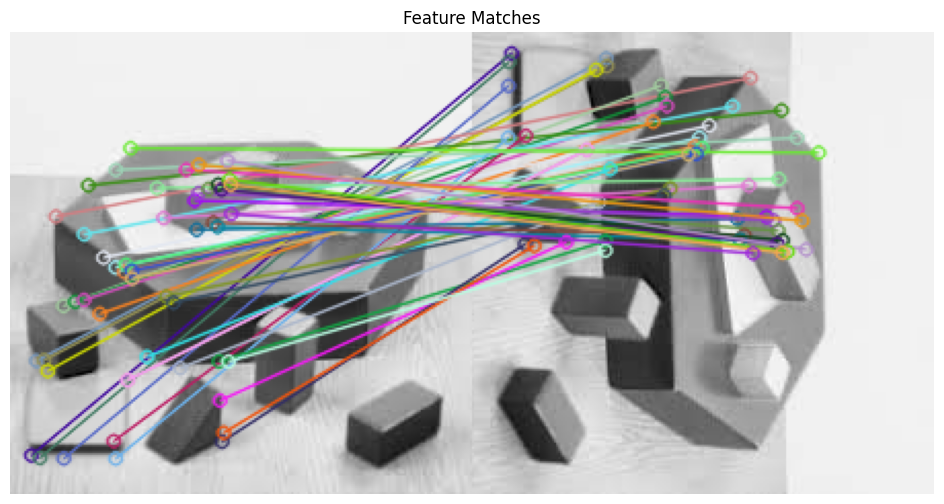
\includegraphics[width=0.6\textwidth]{Lab_3/template/figures/FeatureMatch.png}
    \caption{Correspondencia de características entre una imagen y la misma alterada con cv2}
    \label{fig:feat_match}
\end{figure}



\section*{C.1: Detección de puntos de interés}
\phantomsection
\addcontentsline{toc}{section}{C.1: Detección de puntos de interés}

En esta sección se generarán las funciones necesarias que cubran la detección de puntos de interés y los descriptorpes para las imágenes empleando la transformación SIFT.
La transformación SIFT consta de cuatro pasos principales:

\begin{enumerate}
    \item Detección de extremos en espacio de escalas
    \item Localización de keypoints
    \item Asignación de orientaciones
    \item Generación de los descriptores de keypoints
\end{enumerate}

Cada uno se irá desarrollando con las funciones necesarias para completarlos. De esta forma se comenzará generando el espacio de escalas en el que se evaluarán los extremos

\subsection*{Tarea C.1.1: Filtro gaussiano con cv2}
\phantomsection
\addcontentsline{toc}{subsection}{Tarea C.1.1: Filtro gaussiano con cv2}

Para generar el espacio de escalas que se desea analizar, se debe aplicar un filtrado gaussiano a la imagen original hasta obtener un número de imágenes gaussianas relevante. Para ello, debe desarrollar la función \texttt{generateGaussianImages()} empleando el método \texttt{GaussianBlur()} de la librería cv2.

Como entrada, se recibe una imagenm, y una lista de sigmas que deberá aplicar en el filtrado. Deberá generar tantás imágenes gaussianas como sigmas haya en la lista aplicando el filtro al resultado del filtrado anterior o a la imagen original en primera instancia.

\subsection*{Tarea C.1.2: Generación de espacio de escalas con imágenes gaussianas}
\addcontentsline{toc}{subsection}{Tarea C.1.2: Generación de espacio de escalas con imágenes gaussianas}

Deberá cargar la imagen base de la carpeta de \texttt{data} con cv2 y en escala de grises sin emplear la función \texttt{cv2.cvtColor()}. A continuación, se definen los parámetros iniciales del espacio de escalas, la \textit{sigma} inicial y el número de diferencias gaussianas que se desea generar. Cabe destacar que aunque el mínimo de gaussianas necesarias son 3 para detectar los máximos y minimos en las ventanas de 3x3x3 como se verá más adelante, es posible que no sea suficiente este valor para detectar esos puntos de interés. Por último, emplee el método \texttt{generateGaussianImages()} que ha desarrollado en el apartado anterior.

Como puede observar en el código, se le proporciona el método \texttt{generateGaussianSigmas()} que recibe la \textit{sigma} inicial y el número de diferencias de gaussianas que desea generar. Este método devuelve una lista de valores de \textit{sigma} que deberá aplicar en los filtrados consecutivos para la generación de las imágenes gaussianas. Si quiere generar \textit{n} diferencias de gaussianas, el método le devolverá \textit{n+1} valores de sigma.

\begin{figure}[h]
    \centering
    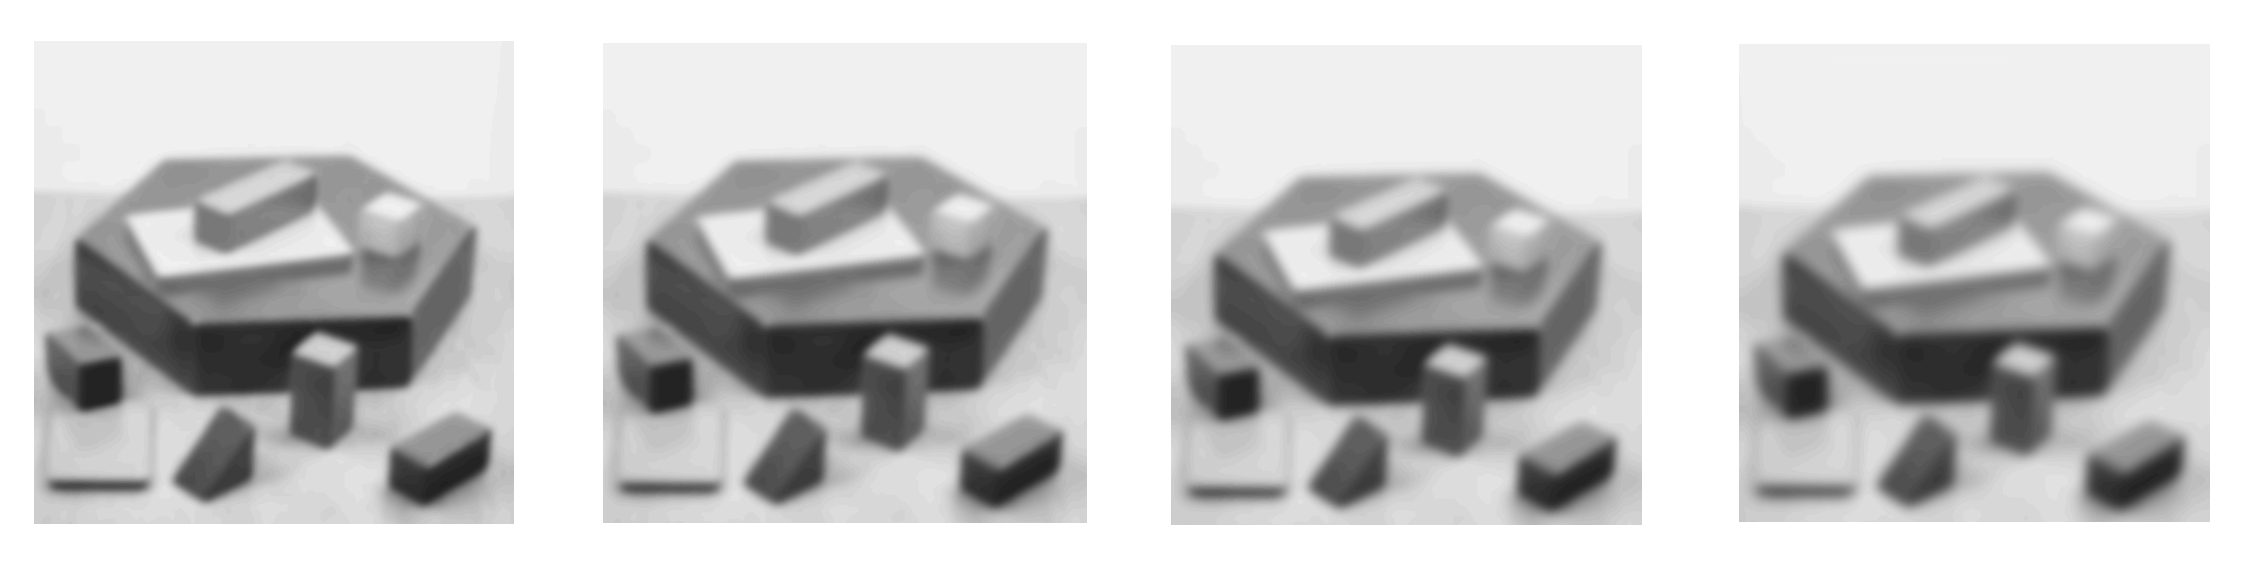
\includegraphics[width=0.8\textwidth]{Lab_3/template/figures/GaussianBlur.png}
    \caption{Resultados esperados de la generación de imágenes gaussianas}
    \label{fig:gauss_blur}
\end{figure}

\subsection*{Tarea C.1.3: Generación de diferencias de gaussianas}
\addcontentsline{toc}{subsection}{Tarea C.1.3: Generación de diferencias de gaussianas}

A partir de la lista de imágenes anteriores, se deberán generar una nueva lista con las diferencias entre las imágenes consecutivas empleando el método \texttt{subtract} de la librería \texttt{cv2}.

\begin{figure}[h]
    \centering
    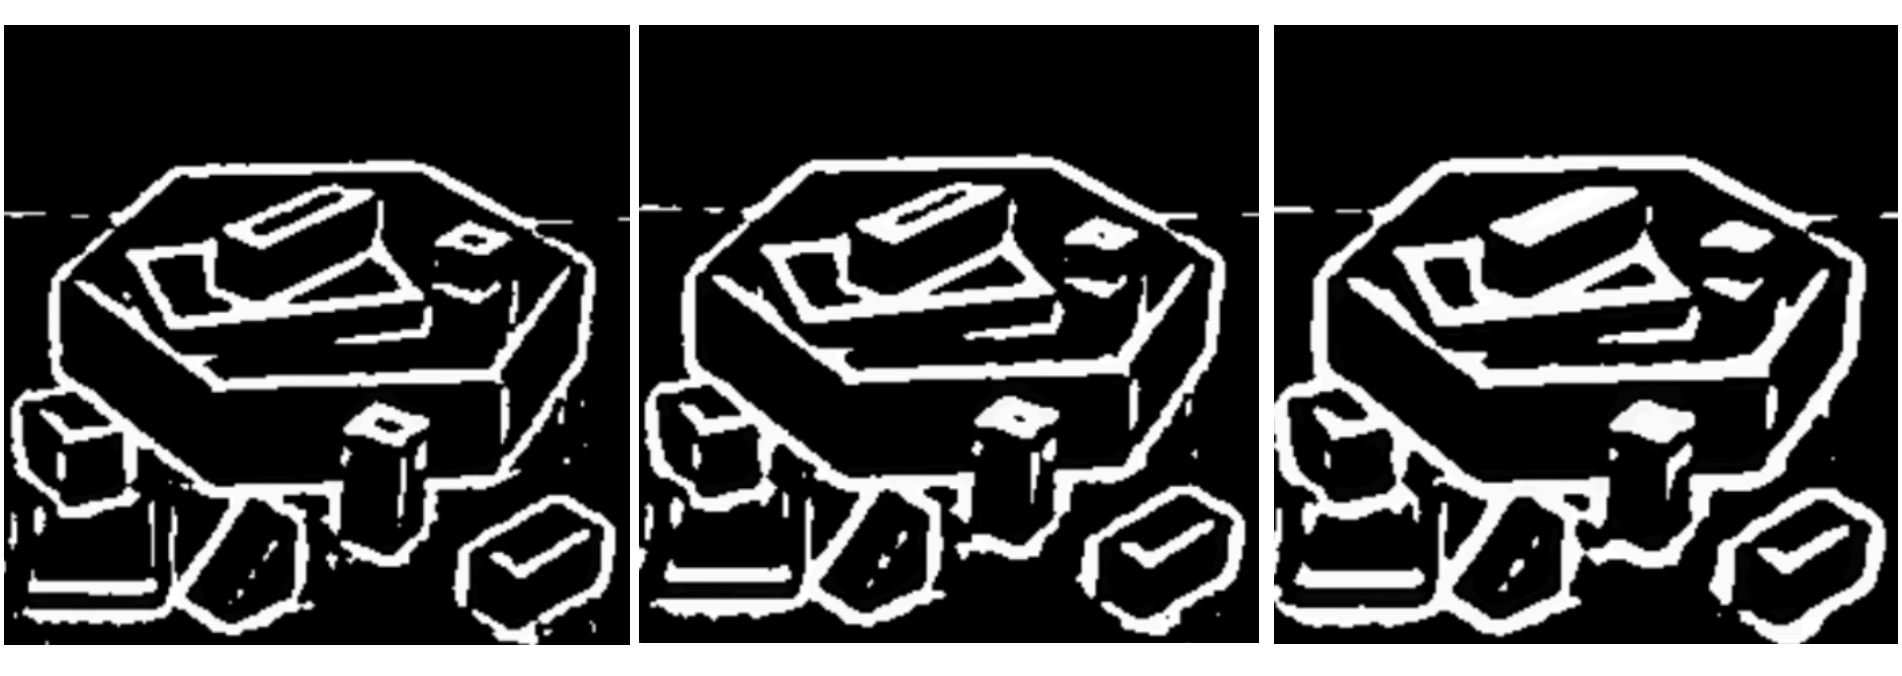
\includegraphics[width=0.8\textwidth]{Lab_3/template/figures/DoG.png}
    \caption{Resultados esperados de la generación de diferencias gaussianas}
    \label{fig:dog}
\end{figure}


\subsection*{Tarea C.1.4: Evaluación de extremos}
\addcontentsline{toc}{subsection}{Tarea C.1.4: Evaluación de extremos}

En esta tarea debe desarrollar la función \texttt{isPixelAnExtremum()} que evalua si el fixel central de una ventana de 3x3x3 es un máximo o mínimo entre sus vecinos y si es superior a un umbral mínimo en valor absoluto. La ventana está compuesta por 3 regiones de 3x3 píxeles cada una que corresponden a regiones de 3 diferencias de gaussianas consecutivas. La función debe devolver \textit{True} en caso de ser un máximo o mínimo y \textit{False} en cualquier otro caso. \textbf{Importante:} Tras el filtrado gaussiano, los píxeles pueden tener valores negativos.

\subsection*{Tarea C.1.5: Localización de puntos de interés y orientación de los mismos}
\addcontentsline{toc}{subsection}{Tarea C.1.5: Localización de puntos de interés y orientación de los mismos}

Empleando la función completada en el apartado anterior deberá completar el desarrollo de la función \texttt{findScaleSpaceExtrema()}.

Primero tendrá que completar el bucle \texttt{for} para obtener en cada iteración 3 diferencias de gaussianas consegutivas y enumerarlas. Tras esto, iterar sobre las coordenadas de estas teniendo en cuenta que deberá mover la ventana de 3x3 a través de toda la imagen y no puede quedar ningún punto de esta ventana fuera de la misma. Complete la llamada a la función \texttt{isPixelAnExtremum()} con los argumentos pertinentes para evaluar si el pixel en las coordenadas de esa iteración es un punto extremo.

Si los píxeles son máximos o mínimos ya te tiene una localización aproximada de los puntos de interés de esta imagen. La función \texttt{localizeExtremumViaQuadraticFit()} refina esta localización teniendo en cuenta elk gradiente y el hessiano y descartando los valores que no tengan el suficiente contraste. Con la localización final se obtiene la orientación del punto de interés gracias a la función \texttt{computeKeypointsWithOrientations()}, del resultado de esta función se tiene el punto de interés definido completamente.

Se recomienda el uso de la función de borrado de duplicados ya que existen puntos de interés que se repitan en el resultado del proceso anterior. Se proporciona al alumno la función \texttt{visualizeKp()} que le permitirá visualizar los puntos de interés en la imagen original.

\begin{figure}[h]
    \centering
    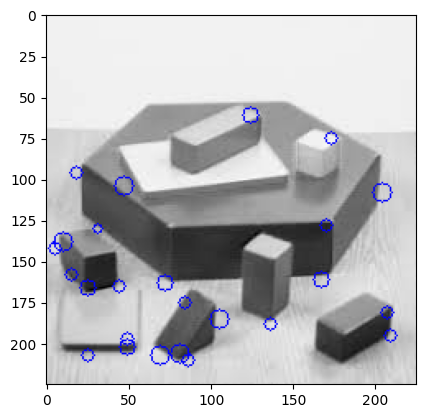
\includegraphics[width=0.4\textwidth]{Lab_3/template/figures/KeypointDetect.png}
    \caption{Resultados esperados de la detección de puntos de interés y orientación}
    \label{fig:KPDet}
\end{figure}

Una vez obtenidos las imágenes gaussianas y los puntos de interés con sus orientaciones se pueden generar los desciptores de las regiones vecinas a los mismos que sea invariante a los cambios en la iluminación y el punto de vista 3D. En esta sesión esto se le proporciona al alumno con la función \texttt{generateDescriptors()}.

\subsection*{Tarea C.1.6: \textit{Pipeline} de generación de puntos de interés y descriptores}
\addcontentsline{toc}{subsection}{Tarea C.1.6: \textit{Pipeline} de generación de puntos de interés y descriptores}

En esta taream el alumno deberá completar la función \texttt{computeKeypointsAndDescriptors()}. Esta función recibe la imagen original, el valor inicial de \textit{sigma} y el número de diferencias de gaussianas que se desee generar. La tarea del alumno es completar la función con los metodos desarrollados en apartados anteriores para obtener el \textit{pipeline} completo de localización de puntos de interés y generación de descriptores.

\subsection*{Tarea C.1.7: Correspondencia de características entre imágenes}
\addcontentsline{toc}{subsection}{Tarea C.1.7: Correspondencia de características entre imágenes}

En esta tarea, el alumno comprobará la capacidad de sistema de localizar las mismas características en una imagen alterada para luego establecer la correspondencia entre las características de la imagen original y la de la alterada. Esto se conseguirá cargando la imagen original y la alterada en escala de grises con la librería de \texttt{cv2}. Después tendrá que hacer las llamadas pertinentes al método desarrollado en el apartado anterior para obtener los puntos de interés y descriptores de ambas imágenes. 

Con estos datos, empleando la función \texttt{matchFeatures()} comprobará la capacidad de establecer la correspondencia entre los puntos de interés de ambas imágenes.

\begin{figure}[h]
    \centering
    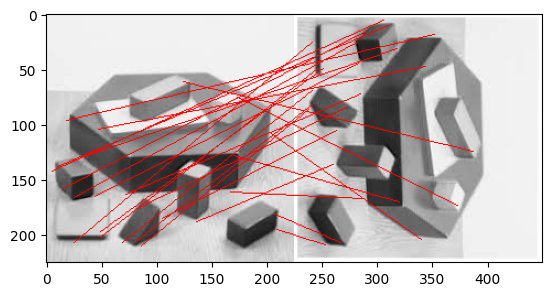
\includegraphics[width=0.8\textwidth]{Lab_3/template/figures/FeatureMatchMine.png}
    \caption{Resultados esperados de la correspondencia de características}
    \label{fig:FMatchEnd}
\end{figure}

Una vez comprendido el funcionamiento de un dectector de puntos de interés y descriptores se anima al alumno a emplear el método propio de la librería \texttt{cv2} como se proporciona en el cuaderno.


\subsection*{Preguntas}
\addcontentsline{toc}{subsection}{Preguntas}

\vspace{5mm}
\begin{tcolorbox}[colback=gray!10, colframe=gray!30, coltitle=black, title=Pregunta C.1: Correspodencia de imágenes propias y evaluación, halign=left]
Con los métodos desarrollados para la extracción de características, haga uso del \textit{pipeline} que ha desarrollado y de el método propio de cv2 con sus propias imágenes. Adjunte los resultados en ambos casos y comparelos extrayendo sus propias conclusiones.
\end{tcolorbox}

\section*{C.2: Bolsa de palabras}
\phantomsection
\addcontentsline{toc}{section}{C.2: Bolsa de palabras}

En este apartado se va a genera una bolsa de palabras a partir de un dataset de entrenamiento y se evaluará con un dataset de evaluación. Para generar la bolsa de palabras, se segirán los pasos descritos en las sesiones de teoría:

\begin{enumerate}
    \item Extracción de descriptores de puntos de interés de las imágenes del dataset
    \item Construcción de diccionario de palabras visuales (K-Means)
    \item Para cada imagen del dataset, generar histograma de ocurrencias de palabras del diccionario
    \item Obtener clasificador utilizando los histogramas de las imágenes del dataset (SVM)
\end{enumerate}

De esta forma, se comenzará con la carga de las imágenes que compondrán los distintos \textit{datasets} para ser procesadas posteriormente.

\subsection*{Tarea C.2.1: Carga de \textit{datasets} de entrenamiento y validación}
\addcontentsline{toc}{subsection}{Tarea C.2.1: Carga de \textit{datasets} de entrenamiento y validación}

Como ayuda, se le proporciona una clase de python llamada \textit{Dataset}. Empleando el método \texttt{load()} de esta clase, cargue los \textit{datasets} de entrenamiento y validación.

\subsection*{Tarea C.2.2: Extracción de los descriptores}
\addcontentsline{toc}{subsection}{Tarea C.2.2: Extracción de los descriptores}

Una vez cargados los \textit{datasets} se puede proceder a extraer los descriptores de las imágenes que poblaran nuestra bolsa de palabras. Estos conformarán las ocurrencias de cada en la bolsa. Para ello, primero deberá cargar las imágenes el \textit{dataset} de entrenamiento con el \texttt{path} de cada una de ellas y hacerlo en escala de grises. Después, empleando los métodos necesarios de cv2 que ha visto durante la sesión, genere los descriptores y guárdelos en una lista.

\subsection*{Tarea C.2.3: Creación del vocabulario}
\addcontentsline{toc}{subsection}{Tarea C.2.3: Creación del vocabulario}

Con la bolsa de palabras llena con los descriptores, se puede proceder a agrupar los mismos en las distintas palabras del vocabulario que se va a generar. Para ello, se va a ejecutar el algoritmo de clusterización de K-Means que agrupará estos descriptores. En esta tarea debe añadir los descriptores de la lista que obtuvo como resultado en la tarea anterior a la bolsa de palabras \texttt{words} que se inicializa en el código y sobre la que ejecutaremos el algoritmo. Fíjese en que se determina el número de palabras deseadas en el vocabulario final con la variable \texttt{vocabulary\_size} y que esto afectará al desempeño del clasificador más adelante.

\subsection*{Tarea C.2.4: Entrenamiento del clasificador}
\addcontentsline{toc}{subsection}{Tarea C.2.4: Entrenamiento del clasificador}

Una vez tenemos las características de las imágenes agrupadas en las palabras, se va a entrenar un clasificador que sea capaz de diferenciar entre estos grupos. Este será un modelo basado en una  \textit{Support Vector Machine}(SVM). Con este clasificador podremos recibir imágenes externas al \textit{dataset} de entrenamiento y clasificarlas en nuestro grupo de palabras.

Para entrenar el clasificador se aporta la clase \texttt{BoW} como ayuda. Añada los argumentos necesarios a los métodos especificados en la celda de código. Compruebe qué argumentos tiene que añadir accediendo al código de la clase proporcionada y analizando los métodos declarados. El modelo final se guardará en el ordenador para su uso más adelante.

\subsection*{Tarea C.2.5: Inferencia en el dataset de entrenamiento}
\addcontentsline{toc}{subsection}{Tarea C.2.5: Inferencia en el dataset de entrenamiento}

Con el modelo entrenado, es hora de ver como trabaja y su desempeño. En este caso la métrica empleada será la precisión y podrá observar la matriz de confusión generada de las predicciones.

Al igual que en la tarea anterior, añada los argumentos necesarios a los métodos especificados en la celda de código.

\subsection*{Tarea C.2.6: Inferencia en el dataset de validación}
\addcontentsline{toc}{subsection}{Tarea C.2.6: Inferencia en el dataset de validación}

Después de extraer los resultados con el dataset de entrenamiento, se tienen que comparar los mismos con los del dataset de validación donde se debería obtener un desempeño inferior.

Al igual que en la tarea anterior, añada los argumentos necesarios a los métodos especificados en la celda de código.


\subsection*{Preguntas}
\addcontentsline{toc}{subsection}{Preguntas}

\vspace{5mm}
\begin{tcolorbox}[colback=gray!10, colframe=gray!30, coltitle=black, title=Pregunta C.2: Cambio de SIFT por KAZE, halign=left]
Ejecute el proceso completo de nuevo cambiando el extractor de características SIFT por KAZEincluido también en la librería de cv2 y en las clases de ayuda proporcionadas. Incluya el código y los resultados de inferencia en entrenamiento y validación
\end{tcolorbox}

\vspace{5mm}
\begin{tcolorbox}[colback=gray!10, colframe=gray!30, coltitle=black, title=Pregunta C.3: Cuantas palabras uso?, halign=left]
Como ha podido comprobar, a la hora de agrupar los descriptores y generar el vocabulario se indica el tamañó del vocabuulario, número de palabras, que se desea. Itere sobre este valor y fíjese en los efectos de este sobre el desempeño final con el dataset de entrenamiento y validación. Incluya como resultados, los valores empleados, la precisión obtenida y las conclusiones sobre el número adecuado de palabras a emplear.
\end{tcolorbox}
\vspace{5mm}

\begin{tcolorbox}[colback=gray!10, colframe=gray!30, coltitle=black, title=\textbf{EXTRA} - Pregunta C.4: En busca de los mejores parámetros, halign=left]
Al igual que ha iterado en la pregunta anterior con el número de palabras, itere con el resto de parámetros como el número de iteraciones para el K-Means, el número de iteraciones para el SVM, el extractor de caractrerísticas... Proporcione el código final con los parámetros de entrenamiento y los resultados obtenidos. El grupo que obtenga mayor precisión en validación recibirá un punto extra en la práctica.
\end{tcolorbox}
